%===================================== CHAP 2 =================================

\chapter{Background}
\label{chap:background}



\section{Concepts}
This section explains some of the essential concepts for this thesis.


\subsection{Reality-Virtuality Continuum} \label{background:Continuum}
In 1996, Paul Milgram described the \textit{Reality-Virtuality Continuum}\cite{milgram1995augmented}. The paper describes in detail the different types of virtuality and reality that exist on this scale, and the major differences that separate them. As Figure \ref{fig:VR_continuum} illustrates the the real world and virtual world are opposite ends of the continuum, with mixed reality (MR) covering the majority, but not including, the fully real and virtual environments. 

The application system developed for this project find themselves at the right hand side of the continuum, as mostly virtual environments, but also within the mixed reality concept.  

\begin{figure}
    \centering
    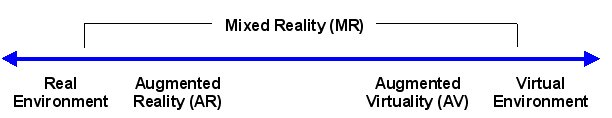
\includegraphics[width=\textwidth]{./fig/background/Virtuality_Continuum_2}
    \caption{The Virtuality-Reality Continuum}
    \label{fig:VR_continuum}
\end{figure}


\subsubsection{Virtual Reality}
The definition of virtual reality has changed over the years, for example when Milgram et al. defined it 1995 \cite{milgram1995augmented} as an environment in which "...participant-observer is totally immersed in a completely synthetic world, which may or may not mimic the properties of a real-world environment, either existing or fictional, but which may also exceed the bounds of physical reality by creating a world in which the physical laws governing gravity, time and material properties no longer hold." D. Guttentag \cite{guttentag2010virtual} later defined it in 2010 as “the use of a computer-generated 3D environment...that one can navigate and possibly interact with, resulting in real-time simulation...".

Although definitions differ, the concept remains the same - a virtual environment which supports navigation and interaction. Today, these environments are often displayed to the user using a head mounted display (HMD), but there exists other ways, including room scale projections.

\subsubsection{Mixed Reality} \label{background:MixedReality}
As with virtual reality, the definition of mixed reality (MR) has changed from when Milgram et al. defined it  \cite{milgram1995augmented} as an environment where "...real world and virtual world object are presented together within a single display...". It can been seen as anywhere on the continuum except on the extrema, see Figure \ref{fig:VR_continuum}. However, the usage of the term MR has been somewhat lose with manufactures such as HP and Microsoft putting it on their headsets or in their desktop application. In the \textit{What is mixed reality?} \cite{microsoftMR} article by Microsoft they describe it as a blend of physical and digital world where the mixed reality spectrum covers and fully includes the physical world and the digital world, unlike the continuum by Milgram et al. which does not, see Figure \ref{fig:MicrosoftSpectrum}.

Although, they are quite similar it is important to note and that for this project we will follow the definition of MR defined by Milgram et al., which means whenever we refer to mixed reality we do not include the fully real- or virtual environment in that reasoning.  

\begin{figure}
    \centering
    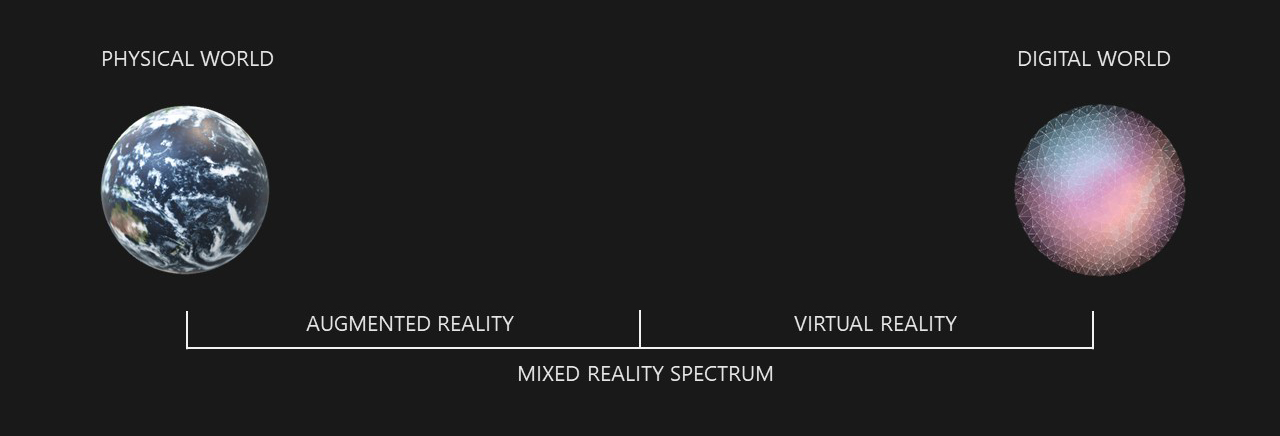
\includegraphics[width=\textwidth]{./fig/background/microsoft_spectrum.jpg}
    \caption{The mixed reality spectrum according to Microsoft \cite{microsoftMR}.}
    \label{fig:MicrosoftSpectrum}
\end{figure}


  
\subsubsection{Immersion and presence} \label{immersionAndPresence}
It is important to note the difference between presence and immersion. While immersion refers to an an objective level of fidelity, which can be measured against the immersion levels of another application, presence refers to a person's subjective feeling of being in a location while physically being in another \cite{slater2003note}. With this project we hope to increase the presence of the user in the virtual workplaces, not necessarily the immersion.

\subsubsection{Social presence}
\label{section:socialPrecence}
Presence refers to the subjective feeling of being somewhere else than you are physically, but it can be split into three types of presence, of which social presence is the most relevant for this paper. Self-presence refers to the feeling of being connected to your virtual body, tele-presence refers to the subjective feeling of being spatially located elsewhere than your physical body, and social presence refers to the feeling of being in the presence of another intelligence. If the feeling of social presence is not high enough, the other part is felt to simply be an artificial entity.

%One of the primary goals of... 
One of the goals of the project is to create a high level of social presence. Social presence was defined by Biocca in a 1997 paper as "\textit{The minimum level of social presence occurs when users feel that a form, behaviour, or sensory experience indicates the presence of another intelligence. The amount of social presence is the degree to which a user feels access to the intelligence, intentions, and sensory impressions of another}\cite{biocca1997cyborg}."

There are several conditions that can affect the social presence of a user, one of which is the visual representation. While it may seem logical to assume that a higher degree of photographic or anthropomorphic realism for avatars would increase the feeling of social presence, studies show that this may not be enough. The two things that seem to be the most important for social presence is the presence of a visual representation and a more behaviourally realistic visual representation. People show increased involvement and engagement when the person they are communicating with is visible at all, or has a profile picture instead of a default picture. While a high degree of photo realism can be used, it will be detrimental if there is not a commensurate increase in behavioural realism\cite{oh2018systematic}.

Interactivity is another part of social presence. Skalski noted that being able to interact with virtual agents increased users feeling of social presence\cite{skalski2007role}. There are also several other aspects that can affect social presence, such as haptic feedback, depth cues, audio quality and display types\cite{oh2018systematic}. 

In general, social presence is at the heart of this paper, and seeing the effects social presence has on the overall presence and what that can do for the overall engagement and experience of the users will be an important part of the project. The hypothesis that an increase in social presence will make the applications more engaging than they are now appears to be supported by the literature, as "...studies show that the vivid perceptions of another person often lead to greater enjoyment and social influence in neutral and positive contexts\cite{oh2018systematic}".







\subsection{Workspace Awareness in Groupware}
When collaborating with others, there are several ways in which we gather information. Many of these are subtle and perhaps not outright obvious, but are important none the less as ways to collaborate efficiently. The awareness of others' location, actions and intentions in regard to the task are referred to as \textit{workspace awareness}.

When working with groupware, workspace awareness is not a given. It must be implemented by developers and rigorously tested to make sure it works well. The developer must explicitly create the forms of interaction and tools to support workspace awareness\cite{gutwin1996workspace}.

In spite of this, one does not need to start entirely from a blank sheet. There are certain elements that make up the core elements of workspace awareness, as seen in tables \ref{table:awarenessPresent} and \ref{table:awarenessPast}\cite{gutwin2002descriptive}. Using these categories as a framework, one can more easily consider what parts are necessary for the workspace you are creating and make decisions based on that.



\begin{table}[!h]

      \centering
        \caption{Elements of workspace awareness relating to the present}
        \begin{tabularx}{\textwidth}{lll}
        \toprule
        Category & Element & Specific Questions\\
        \midrule
        Who & Presence & Is anyone in the workspace?\\
         & Identity & Who is participating? Who is that?\\
        \vspace{0.2cm}
         & Authorship & Who is doing that?\\
        
        What & Action & What are they doing?\\
         & Intention & What goal is that action part of?\\
        \vspace{0.2cm}
         & Artifact & What object are they working on?\\
        
        Where & Location & Where are they working?\\
         & Gaze & Where are they looking?\\
         & View & Where can they see?\\
         & Reach & Where can they reach?\\
        
        \bottomrule
        \label{table:awarenessPresent}
        \end{tabularx}
\end{table}

\begin{table}[!h]
      \centering
        \caption{Elements of workspace awareness relating to the past}
        \begin{tabularx}{\textwidth}{lll}
        \toprule
        Category & Element & Specific Questions\\
        \midrule
        How & Action history & How did that operation happen?\\
        \vspace{0.2cm}
         & Artifact history & How did this artifact come to be in this state?\\\vspace{0.2cm}
        When & Event history & When did that event happen?\\\vspace{0.2cm}
        Who (past) & Presence history & Who was here, and when?\\\vspace{0.2cm}
        Where (past) & Location history & Where has a person been?\\\vspace{0.2cm}
        What (past) & Action history & What has a person been doing?\\
        \bottomrule
        \label{table:awarenessPast}
        \end{tabularx}
\end{table}

Table \ref{table:awarenessPresent} describes the elements of workspace awareness that relate to the present, while table \ref{table:awarenessPast} refers to the past. When working together in a workspace, there are three major categories of perception that a person can employ to quickly orient themselves in the workspace, namely "Who", "What" and "Where". By observing the other participants of the workspace, either consciously or subconsciously, a person will be able to infer who's doing what, what they are doing and where they are working. In certain groupware, like a shared text editor, this would be solved by showing the caret of other users to indicate \textit{where} they are currently working, as well as icons to indicate \textit{who} is in the workspace. For a VR application, there is a whole new range of affordances available to the user, and one needs to tackle the issue of a shared workspace differently than one would in a non-immersive application.


In the versions of the applications made for one user at a time, the guidance counsellor/operator would have to explain how things like tasks worked and where objectives were located without existing in the same virtual space. This disconnect proved disadvantageous and ineffective, and the presence of the user suffered due to the disconnect between the virtual space they were in and the instructions coming in from outside of this space. Enabling workspace awareness with others, be it other users or supervisors, enhances several activities. A brief summary of these can be seen in table \ref{table:awarenessActivity} \cite{gutwin2002descriptive}. 

Perhaps the most significant activity that can easily be enhanced with VR is \textit{simplification of communication}. This refers to the deictic gestures like pointing and waving, interacting with artefacts to show other users, etc. These interactions will be included as a byproduct of achieving the level of immersion deemed necessary by us, the IMTEL lab and NAV. The other activities are also important, allowing greater ease of communication and planning for the users and significantly increasing their awareness of the current status of the work being done, and how they can best assist each other.

\begin{table}[!h]
      \centering
        \caption{Summary of the activities in which workspace awareness is used}
        \begin{tabularx}{\textwidth}{l X}
        \toprule
        Activity & Benefit of workspace awareness \\
        \midrule
        \vspace{0.2cm}
        Management of coupling & Assists people in noticing and managing transitions between individual and shared work.\\
        \vspace{0.2cm}
        Simplification of communication & Allows people to the use of the workspace and artifacts as conversational props, including mechanisms of deixis, demonstrations, and visual evidence.\\\vspace{0.2cm}
        Coordination of action & Assists people in planning and executing low-level workspace actions to mesh seamlessly with others.\\\vspace{0.2cm}
        Anticipation & Allows people to predict others’ actions and activity at several time scales.\\\vspace{0.2cm}
        Assistance & Assists people in understanding the context where help is to be provided.\\
        \bottomrule
        \label{table:awarenessActivity}
        \end{tabularx}
\end{table}



\subsection{Computer-Supported Collaborative Learning} \label{CSCL}
\label{section:CSCL}
The field of Computer-Supported Collaborative Learning (CSCL) is highly relevant to the task at hand. CSCL is a multi-disciplinary field seeking to use technology to empower users to collaborate and learn together \cite{stahl2006computer}.  It is also important to make the distinction between \textit{collaboration} and \textit{cooperation}. Where as cooperation is defined by Dillenbourg as the division of work into subtasks which eventually are pieced together to form a final result, he defines collaboration as working "together" \cite{dillenbourg1999you}.

The concept can roughly be split into two parts. Namely, the computer support and the collaborative learning. CSCL is inherently social, and the technology must strive to support that. Technology also offers unique opportunities that need to be catered to, rather than attempting to create something that does not take advantage of these opportunities, or tries to solve problems for which the technology is not suited.

The collaborative learning aspect is interesting because not only do you use collaboration to increase the learning effect, the learning itself is constituted of the interaction between the participants\cite{stahl2006computer}. That is to say, even should you attempt to learn something on your own, the knowledge you gain is inherently different from the knowledge one would gain through collaboration.


CSCL stresses collaboration among the users. When used properly, the users will learn together, motivate each other and gain a richer learning experience in general through collaborative learning.

This sentiment is further reinforced in a 2017 paper by Greenwald et al. \cite{greenwald2017technology}, which states that "\textit{...direct mutual exchange about the digital content increases their relevance for users and supports mutual confirmation. Our studies show that users can build on body language and deictic gestures just as they do with real world objects and that collaborative visual search increases the understanding of all involved users.}" This supports the motivation that applying collaborative learning to the Virtual Internship project will yield positive effects. The inclusion of VR allows the users to apply deictic gestures, use demonstrations and coordinate better. In general, it is a good way to increase workspace awareness, and will support several of the activities listed in Table \ref{table:awarenessActivity}.

\subsection{Collaboration in Virtual Reality}
There are many upsides to collaboration in virtual reality. In the CSCL section, the concept of learning through interaction was discussed, and how that learning can be fundamentally different from normal learning. Through VR, one can transfer a lot of the usual interactions performed when working with other in the real world directly, allowing for better efficiency and larger presence for the users\cite{greenwald2017technology}. While the procedure of creating a virtual collaborative can be both expensive and lengthy, it is a one-time cost where the benefits can often offset this cost.  A 2017 study showed that using a collaborative virtual environment made users more involved and immersed in their task. The testers also reported that they enjoyed using the tool as well, showing that there are a lot of positives to using virtual reality in this way. They also reported that they experienced a greater workload, so usage may have to be managed so as to not burn users out\cite{madathil2017investigation}.

%\subsection{Collaborative Virtual Environments for Supporting
%Learning Communities}
%Monica Divitini and Ekatarina paper 

\subsection{Learning in Virtual Reality}

A literature review in 2015 found that the uses for virtual reality in education were many, stating that "Immersive VR can offer great advantages for learning:  [...] it supports training in a safe environment avoiding potential real dangers and [...] it increases the learner's involvement and motivation..." \cite{freina2015literature}. While there are a general consent among the scientific community that virtual reality can contribute to educational efficacy there are some aspects to consider when developing VR applications for educational use. Roussos et al. describes several dimensions in relation to virtual reality and learning including \textit{technical}, \textit{orientation}, \textit{affective}, \textit{cognitive} and \textit{pedagogical} aspects \cite{roussos1999learning}, as seen in Table \ref{table:awarenessAspects}.



\begin{table}[!ht]
      \centering
      \caption{Summary of the aspects defined by Roussos et al. \cite{roussos1999learning} }
        \begin{tabularx}{\textwidth}{l X}
        \toprule
        Aspect \hspace{1.5cm} & Description \\
        \midrule
        Technical & Usability regarding the interface, software and hardware.
        \vspace{0.2cm}
        \\
        Orientation & Navigation, spatial orientation, presence, immersion and feedback. 
        \vspace{0.2cm}
        \\
        Affective & User engagement, and confidence in the virtual environment.
        \vspace{0.2cm}
        \\
        Cognitive & Internal concepts through the users learning experience.
        \vspace{0.2cm}
        \\
        Pedagogical & Gain knowledge about the environment and concepts being thought.
        \vspace{0.2cm}
        \\
        \bottomrule
        \label{table:awarenessAspects}
        \end{tabularx}
\end{table}

\subsubsection{Career Guidance}
Due to the collaboration with NAV, the expertise in career guidance that NAV has available is available to us, allowing for easier exploration of possibilities in the field. Coupled with available papers, there are considerations that need to be accounted for. According to the literature, the most popular method of career guidance when using computer supported career guidance appears to be individual counselling, followed by classroom and group counselling. They are also mostly used as complementary systems in the counselling process\cite{sampson1987computer}. This lines up well with what NAV has described, and needs to be considered for how the application is developed. 



\subsubsection{Workplace Training}
The use of virtual reality for workplace training is at the core of this project. Previous studies have shown that there is a strong desire for virtual reality workplaces to be applied on a larger scale, both from job seekers and welfare professionals \cite{prasolova2019empowering}. While these applications are being used to some degree, so far it has mostly been for specialised industries or purposes like safety and hazard training. Using the applications to help job seekers enter the workforce has however been less pervasive. 

\subsubsection{Experiential Learning}
Experiential learning refers to learning by doing. Kolb described a more specific 4-step learning model which proposes a cycle of experiential learning\cite{kolb1974toward}. 

\begin{figure}
    \centering
    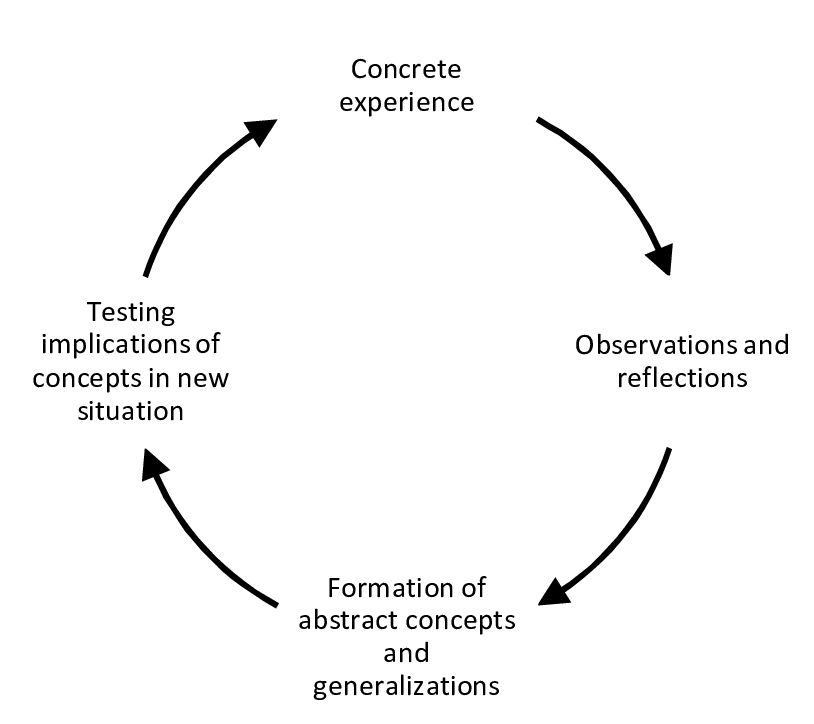
\includegraphics[width=0.7\textwidth]{./fig/background/kolbModel.png}
    \caption{Kolb's experiential learning cycle \cite{kolbModel}.}
    \label{fig:KolbModel}
\end{figure}

The model, as seen in Figure \ref{fig:KolbModel}, describes what Kolb meant constituted experiential learning. To explain the model starting at the top, the person attempting to learn would first gain some form of concrete experience by doing or seeing. Based on this experience, they have to reflect on what just happened and use their observation and reflections to create a new plan based on what worked, and what did not. They can then test these new concepts and again gain new concrete experience, starting the cycle over again.

While the goal of the project is not necessarily training users for a specific workplace, or even preparing them for it, there are many aspects of experiential learning that are useful either way. When considering the target audience for the project, it is important to remember that one of the goals is to increase their self-efficacy and improve their ability to make educated choices about what type of work they want to pursue, Through the use of experiential learning in virtual reality, users are able to try their hand at different scenarios without fear of failure or messing up. This allows them to gain more confidence in their own aptitude for work, and has seen positive reactions \cite{fominykh2019immersive} \cite{prasolova2019empowering}. A 2015 study used collaborative experiential learning in VR to proactively reduce safety hazards in a workplace, and participants agreed that VR was good fit for experiential learning \cite{le2015social}.

\subsubsection{Tutoring}
For those struggling to enter the workforce, it is important that they are able to get the proper impression of a workplace. If more time is spent failing certain tasks rather then organically exploring the tasks at hand, the participant may be discouraged from trying more. Having a tutor or another similar figure present to help keep them on track can be quite beneficial as long as they follow some basic tutoring principles, according to a study by Douglas C. Merill in 1995 \cite{merrill1995tutoring}.

\subsection{Gamification}
Gamification has been a common practice of enhancing a service by including game design principles in a non-game context in order to add value and thereby encourage the user to complete tasks which might seem less interesting on their own. A study by Hamari et al. \cite{hamari2014does} showed that the process yields positive effects and concludes that gamification methods does work.

The IMTEL lab has used gamification principles in most of their Virtual Internship projects as a mean to engage its users. Although these applications use game elements in workplace tasks and situations it is important to note their primary use is \textit{not} to entertain or learn how to do certain tasks but to inform and let users (eg. young job seekers) experience the various workplaces.      

\subsubsection{Serious Games}
Serious games is a subsection of games that do not hold entertainment as their core principle. B. Sawyer defines serious games as "any meaningful use of computerised game/game industry resources whose chief mission is not entertainment." \cite{sawyer2007serious}.
They can be made to tell a story, educate players about a topic or serve as an immersive way to explore a location otherwise inaccessible \cite{susi2007serious}. They offer a way to use gamification principles directly in an application, but even so, they differ somewhat from normal games when it comes to development and game play. According to Zyda \cite{zyda2005visual}, and illustrated in Figure \ref{fig:seriousGames}, serious games has an additional pedagogical component which is one of the aspects identified by Roussos et al. in relation to virtual reality and learning, see Table \ref{table:awarenessAspects}.   

\begin{figure}[!ht]
    \centering
    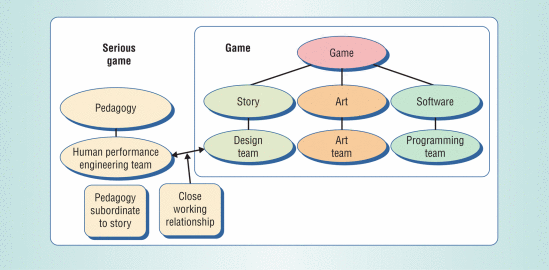
\includegraphics[width=0.9\textwidth]{./fig/background/seriousGames.png}
    \caption{Differences between serious games and game according to Zyda \cite{zyda2005visual}.}
    \label{fig:seriousGames}
\end{figure}

Using serious games for training and education comes with few requirements. For the user to gain anything, it is important that they can gain feedback and be properly assessed. They must also be set up properly to offer the correct level of challenge. Too little, and the player loses interest, while too much difficulty can cause anxiety and stress \cite{de2014serious}. Prasolova-Førland et al. \cite{prasolova2019empowering} recommends care should be taken to balance the educational purpose and entertainment aspects when developing applications for career guidance.

\subsection{Immersive Job Taste}
The IMTEL lab has developed the concept \textit{immersive job taste} as part of the ongoing NAV  project. The concept is designed as a mean to provide a virtual and interactive experience of various occupations with elements of workplace training \cite{fominykh2019immersive}. The target audience for immersive job taste is  young job seekers, e.g. unemployed high school students, with the aim of giving the unemployed a look and experience a different occupations so that they can get a feeling of the daily activities and atmosphere so that they could perhaps avoid wrong career decisions. 

According to Fominykh and Prasolova-Førland \cite{fominykh2019immersive} this concept can make job searching more motivating and provide a more accurate image of a workplace compared to text descriptions. In their research paper confirms that immersive and gaming technologies used in immersive job taste applications contributes to an engaging alternative for young job seekers \cite{fominykh2019immersive}. The concept has also seen recognition from the world beeing awarded in EuroVR 2018 conference for best demo  and was a breakthrough finalist in AWE (Augmented World Expo) 2018 \cite{euroVR} \cite{aweAwards}.



\section{Technologies}
\label{sec:technologies}
This section briefly explains some of the main technologies and frameworks that were used during the development of the artefacts necessary for the projects. 

\subsection{Git}
Git is a version-control-system for collaborative software development work. It makes it easy for multiple participants to work together on single project, and abstracts away a lot of the work involved in merging multiple pieces of code together. For this project we used GitLab \cite{GitLab} as Git-repository manager since the IMTEL lab has their own codebase there. To make Unity work with Git we needed to configure Unity for version control adding specific \textit{.gitignore} settings and using Git LFS (large file system) with corresponding \textit{.gitattributes} settings so that Git tracks large files but keep them out of the GitLab repository. 

\subsection{Unity}
\label{section: untiy}
Unity is one of the most common game development engines used recently \cite{unity}. It is free to use, has a large community and a rich assets store. Unity allows for both 2D and 3D game development with support of physics, advanced graphics rendering and has basic and complex game objects ready to use. As this project contributes to an already established project, the same tools need to be used. Unity allows for quick editing of a scene, and provides a powerful toolset within its layers for developers. Scripting can be done with the C\# or JavaScript coding language and it integrates well with numerous frameworks and plugins.

\subsubsection{Other considerations: Unreal Engine 4}
The other alternative to Unity for VR developments is the Unreal Engine 4 developments suite. It delivers real-time technology and provides an solid foundation for demanding applications across multiple platforms \cite{unrealEngine}. Unreal Engine 4 offers highly advanced visuals but has generally been considered to have a steeper learning curve than compared to Unity. It uses C++, a high level programming language. As mentioned in Section \ref{section: untiy} previous applications has been made using Unity so using Unreal would disallow the use of existing code without rewriting it.       

\subsection{Virtual Reality SDKs}
\label{section:sdks}
For developing VR applications in Unity there exists several software development kits (SDKs) including SteamVR, Oculus and Windows Mixed Reality which is used for connecting with the VR hardware and enables support for building applications for targeted devices.  

% \footnote{https://docs.unity3d.com/Manual/XRPluginArchitecture.html}

Previous Virtual Internship development at the IMTEL lab has used SteamVR which is mainly target for HTC Vive but is fully compatible with other HMDs including Oculus Rift and Touch. For this project OpenVR and SteamVR is chosen as OpenVR enables support for building applications for OpenVR/SteamVR supported devices (eg. most devices at the IMTEL lab). Using OpenVR we can target any platform where SteamVR as, since SteamVR is an implementation of OpenVR, but it also ensures we are not limtied to SteamVR devices.  Figure \ref{fig:vr_sdk} describes the arrangement of the SDKs in this project. The greyed out boxes are SDKs not used in this project, and the green (OpenVR) and red (SteamVR) are SDKs and APIs used in the VR application. As illustrated in the figure we target the SteamVR API in our application but it uses OpenVR which is why it wraps the SDK.

\begin{figure}[!ht]
    \centering
    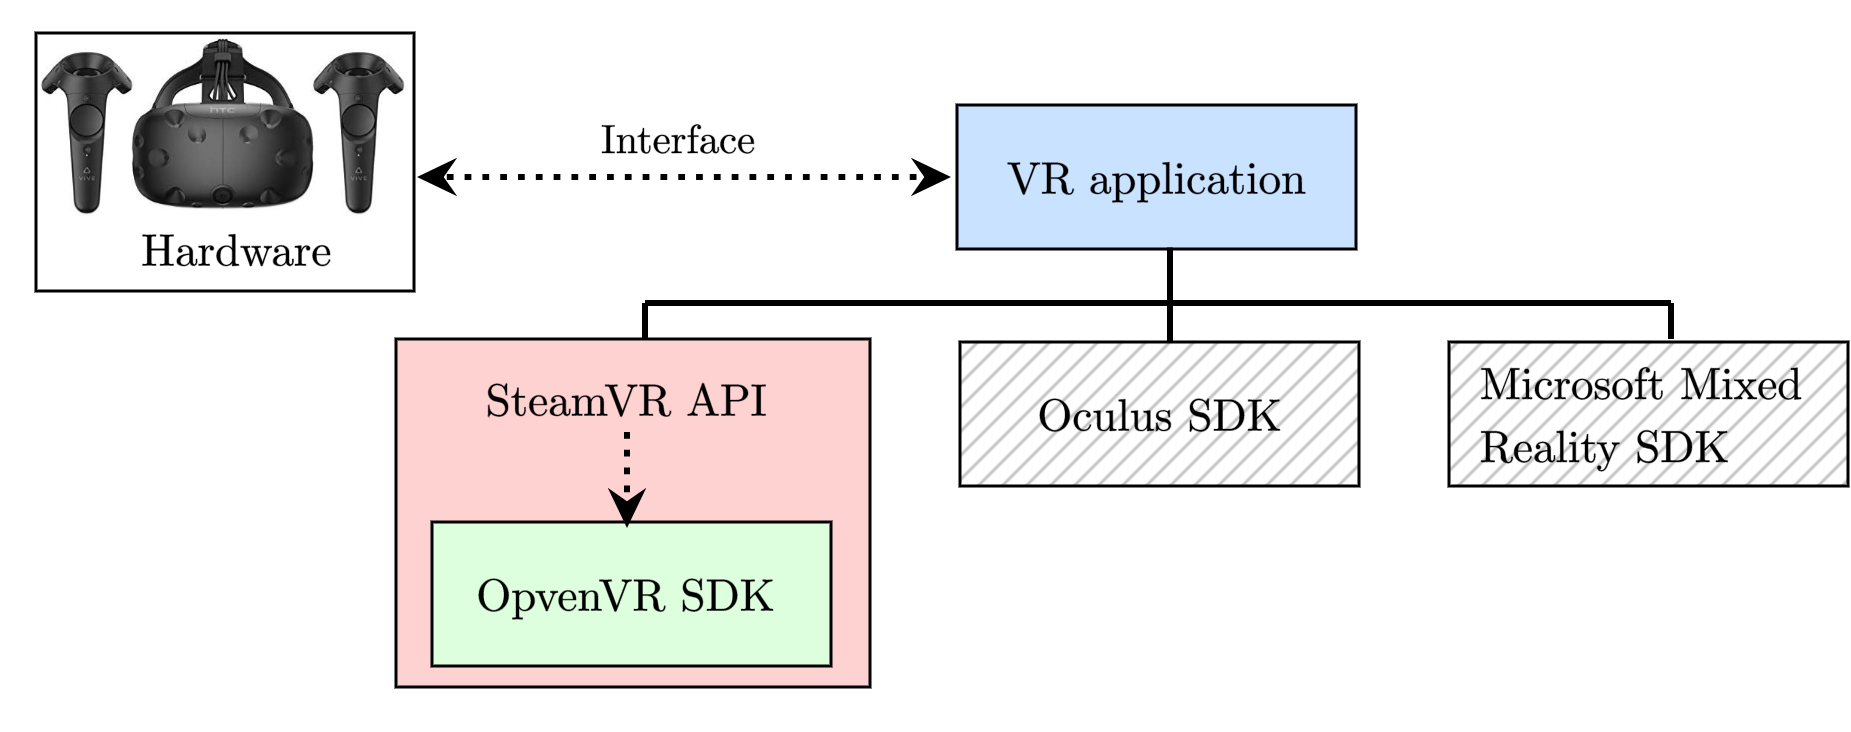
\includegraphics[width=0.9\textwidth]{./fig/background/VR_sdk.png}
    \caption{Illustration of virtual reality SDKs their connection to the application and VR hardware. }
    \label{fig:vr_sdk}
\end{figure}

\subsubsection{OpenVR}
OpenVR is an SDK and API distributed by Valve Corporation that allows access to VR hardware from multiple manufactures like HTC, HP and Oculus. It functions as a interface between the software and hardware \cite{openVRsdk}. SteamVR implements the OpenVR application programming interface (API).  

\subsubsection{SteamVR}
SteamVR is an API and runtime distributed by Valve Corporation. It makes development for VR significantly easier, in that we only need to target the API, and it will make it work for all the major VR headset brands without any extra effort. It also handles input from headsets, and translating the controller input to a fully animated controller inside the application \cite{steamVR}\cite{steamVRAPI}.

\subsection{PUN2 - Photon Networking}
\label{section:pun2}
Photon is a multiplayer game development framework that enables fast and easy setup of a multiplayer server and matchmaking. Specifically, their own wrapper of the framework for Unity, Photon Unity Networking (or PUN) can be imported directly into a Unity project and work seamlessly from there with basic coding required to function. While the base level of functionality is quite simple, considerable work is required to make it fit more advanced certain applications \cite{PUN}. PUN2 includes specific features like callbacks, interfaces, components to synchronise GameObjects and Remote Procedure Calls (RPCs). It uses the client-server architecture, a highly common and used distributed model for networked related communication as illustrated in Figure \ref{fig:ClientServer}, for tasks as matchmaking and synchronisation of data between all clients. 

Take for example a remote procedure call (RPC) or an data stream writing procedure for the updated position of an GameObject. Here the data flows from one client to the PUN2 server using the network (i.e. internet) where it is processed and is sent back to all or specific clients where the GameObject is transformed with its new position (x,y,z coordinates in 3D space). In this project we have configured the application to use servers located in in Europe for a boost in performance and reduced network connectivity related issues. PUN2 also allows to target specific specific clients for RPC calls (see Section \ref{subsec:Optimisation} for more). 

\begin{figure}[!ht]
    \centering
    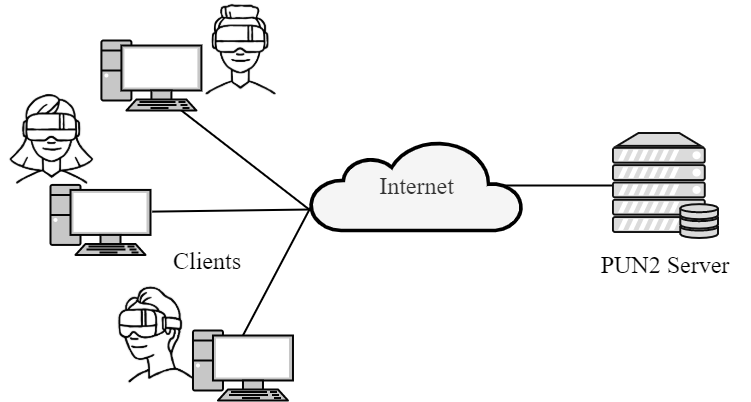
\includegraphics[width=0.8\textwidth]{./fig/background/ClientServer.png}
    \caption{Illustration of client-server architecture used for this application. }
    \label{fig:ClientServer}
\end{figure}

The framework operates on an application/version system. For every program you intend to create and use with Photon, you need to register with Photon as its own application. You can then use this to watch oversee traffic, manage subscriptions, etc. Each application also supports versioning. If two players running the same program have different versions of it, as dictated by the \textit{GameVersion} variable, they will not be able to connect to each other, even if they are on the same application ID. With this, it can be ensured that players will only connect to those on the same version, hindering serious bugs from appearing due to differences in code or scenes.

Photon comes with several features straight out of the box, including matchmaking, in-room communication and dedicated servers. This makes it well suited for creating the required artefacts for the project. Features can be customised as needed, and while one can use the provided example scripts for basic game objects, they do not properly account for all the logic a game object can contain. In most cases, a custom script implementing the API has to be created to cover the needed functionality. As mentioned earlier, one of the artefacts of the project is planned to be a general platform which can be used to develop new projects without needing to do the more basic setup of Photon every time. This would include functionality like voice chat, lobbies, launchers and avatar functionality.

It is therefore important that sufficient time is set aside to not only learn the framework, but also create general solutions that can then be refined in more specific scripts on a per-need basis and embedded in future and existing workplace applications.



\subsection{VR Hardware}
A VR system consists of three major hardware components. As seen in figure \ref{fig:vrHardware} these are the input and output devices (I/O devices) and the VR engine (computer system) \cite{bamodu2013virtual}.  
Input devices includes devices which transmits user actions to the VR engine so that the system can make appropriate actions. This can include headset position data from tracking sensors or simple button presses from the controllers. The VR engine has the responsibility of displaying 3D models through computing tasks such as physics calculations and rendering. Feedback from the engine are sent to the output devices to simulate the virtual environment such as visual and sound.         

\begin{figure}[!ht]
    \centering
    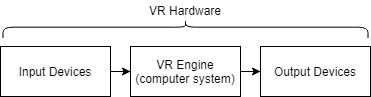
\includegraphics[width=0.6\textwidth]{fig/background/vrHardware.png}
    \caption{The hardware components of a VR system.}
    \label{fig:vrHardware}
\end{figure}

\subsubsection{Displays}
According to Alexander et al there are three different types of displays used for virtual reality . \cite{alexander2017virtual}. They allow a varying degree of immersion and being involved in the synthetic environment \cite{alexander2017virtual}. Figure \ref{fig:vrDiplays} shows the different types which includes handheld, projection and head-mounted display. For this project we will only use head-mounted displays as they give the user a high immersive experience and is already used by previous workplace projects.  


\begin{figure}[!ht]
    \centering
    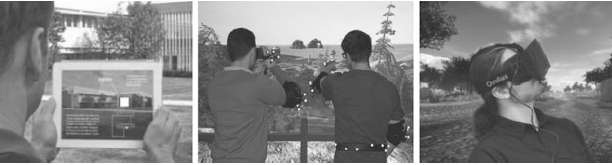
\includegraphics[width=0.9\textwidth]{./fig/background/vrDisplays.PNG}
    \caption{Different types of VR: handheld, projection and head-mounted display \cite{alexander2017virtual}.}
    \label{fig:vrDiplays}
\end{figure}



\subsubsection{Head-mounted display}
Most virtual reality headsets are head-mounted devices that has separate images for each eye. This is a technique known as stereoscopy which creates the illusion of depth from images in order to provide a virtual reality experience. Commonly virtual reality headset systems comes with speakers, microphone, tracking sensors and game controllers. These systems tracks position of the player and the headset using the sensors which enables the program to correctly display part of game scenes relative to the angle and position of the head-mounted display (HMD).

Head-mounted displays gives a high feeling of immersions but there are important considerations in terms of display and hardware to be aware of as it can greatly effect the experience of the user. These are described in the Table \ref{table:hmdSpecs}. HMDs provides a vivid and immersion full experiences however they can also have negative side effects like motion sickness. Reports shows that many users transition from a pleasurable sense of immersion to a high sense of discomfort, disorientation, and nausea \cite{munafo2017virtual}. 

\begin{table}[!ht]
      \centering
      \caption{Important specifications for head-mounted displays to consider.}
        \begin{tabularx}{\textwidth}{l X}
        \toprule
       Specification & Description                                                                           
       \\ 
       \midrule
       \vspace{0.2cm}
        Resolution & The number of pixels used for the display. The more pixel the higher the resolution and thus the details in game providing a more realistic experience.                                   
        \\
        \vspace{0.2cm}
        Refresh rate & How many frames the display can display per second. The higher the refresh rate the smoother the experience is. To avoid motion sickness in VR it is recommended to have a minimum of 90 Hz. 
        \\
        \vspace{0.2cm}
        Field of view (FOV) & How much the user can see of the virtual world. The higher the field of view the more the user can see without rotating the head. A narrow FOV can make the user feel like they are looking at a screen through binoculars.
        \\
        \bottomrule
        \label{table:hmdSpecs}
        \end{tabularx}
\end{table}


Since this thesis uses OpenVR and SteamVR we are not limited to the development of software for specific head-mounted displays. The IMTEL lab offers several modern HMDs including HTC Vive Pro, Valve Index, HP Reverb Mixed Reality and numerous Oculus headsets. The main difference between these HMDs is the use of \textit{base stations}, i.e. wall mounted tracking sensors. HTC Vive Pro (seen in Figure \ref{fig:htcVivePro}) uses these sensors, whereas the HP Reverb (seen in Figure \ref{fig:hpReverb}) does not. Instead it tracks controllers and position using built in sensors in the headset. This is useful when performing test outside the IMTEL lab as there is no need to use base stations.   

\begin{figure}[!ht]
    \centering
    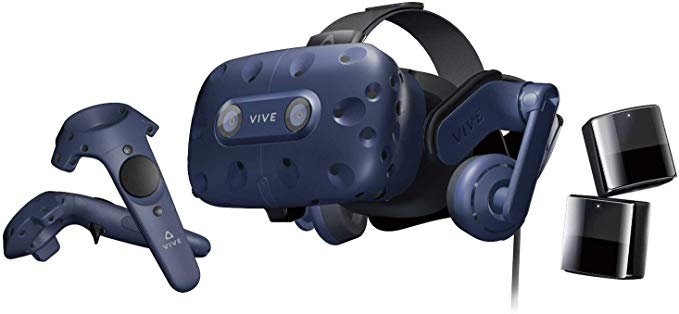
\includegraphics[width=0.6\textwidth]{./fig/background/htcVivePro.jpg}
    \caption{HTC Vive Pro with controllers and base tracking stations.}
    \label{fig:htcVivePro}
\end{figure}

\begin{figure}[!ht]
    \centering
    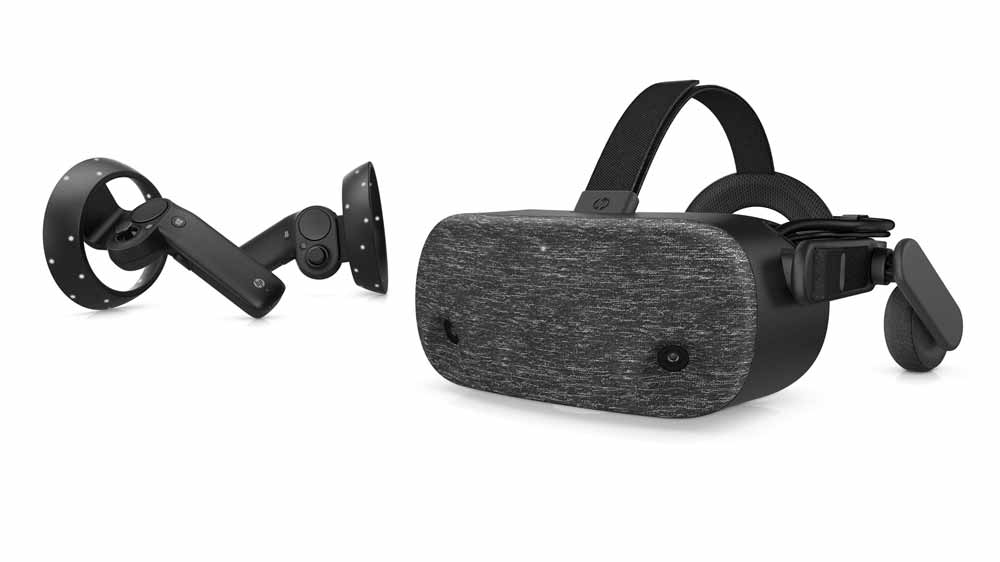
\includegraphics[width=0.6\textwidth]{./fig/background/hpReverbPro.jpg}
    \caption{HP Reverb Mixed Reality with controllers.}
    \label{fig:hpReverb}
\end{figure}


\cleardoublepage